\chapter{Fejlesztői dokumentáció}

	\section{Megvalósítandó feladat}
	
	A program előre megadott alappontok beszúrásával, az alappontokon mért adatokkal számoljon. Radiális bázisfüggvények eltoltjai megfelelő lineáris kombinációjának meghatározása által színezze be a térkép teljes felületét, ezzel közelítést adva az alappontok közti területek hőmérsékletére. Ehhez a részhez lesz szükségünk a matematikai eszközökre, hogy gyorsan és pontosan határozzuk meg a térképet. Nyújtson lehetőséget a színskála tetszés szerinti megválasztására. Ehhez, egyszerű lineáris színátmenetet használok a két alapszín közti értékek számításához. Továbbá háromdimenziós nézet funkció megvalósítása is cél, ahol térbeli ábrázolását láthatjuk az illesztett függvénynek. A lehelyezett alappontok pozícióját lehessen menteni, az adatok későbbi használatának megkönnyítése végett, emellett lehetőséget adunk a színskála mentésére is.
	
	\subsection{Használati esetek}
	
	A program követelményleírása szerinti használati esetdiagram, ahol a lényeges funkciók kerülnek ábrázolásra, melyeket a felhasználó elér és használhat futás közben.
	\begin{figure}[ht]
		\centering
		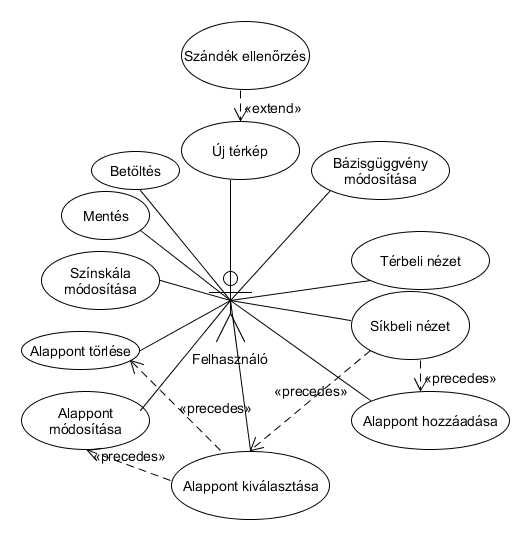
\includegraphics[scale=0.9]{developer/hasznalati_esetdiagram.png}
		\caption{Felhasználói esetdiagram}
	\end{figure}
	
	\subsection{Felhasználói történet táblázat}
	
	A táblázatban a megvalósítandó program funkcióinak részletes bemutatása szerepel felhasználói szemszögből. A követelmény szerinti lehetséges esetekre kitérve a program válaszát láthatjuk az adott szituációkban. A felhasználói eset alatt találhatók a leírásban szereplő funkciók nevei. A leírás alatt pedig egy GIVEN-WHEN-THEN hármas mutatja minden pontnál, hogy az adott programállapotban, a program, felhasználói beavatkozásra, milyen műveletet hajt végre. Jelen esetben az angol szavakat ADOTT-AMIKOR-AKKOR szavakra cserélem az értelmezés megkönnyítése miatt.
	
	\singlespacing
	\begin{longtable}{ |c|m{0.26\linewidth}|c| } 
		
		\hline
		\textbf{\#}  & \textbf{Felhasználói eset} & \textbf{Leírás}\\
		\hline
		{\textbf{1.} } & \textbf{Alkalmazás indítása} &
		{\renewcommand{\arraystretch}{2}
			\begin{tabular}{ c|m{0.45\linewidth} }
				ADOTT & Az alkalmazás Windows 7 vagy újabb operációs rendszeren telepítve van, \\ 
				\hline
				AMIKOR & alkalmazás indítása, \\ 
				\hline
				AKKOR & megjelenik az üres vászon.\\ 
		\end{tabular}}  \\	
		\hline
		{\textbf{2.} } & \textbf{Kilépés} &
		{\renewcommand{\arraystretch}{2}
			\begin{tabular}{ c|m{0.45\linewidth} }
				ADOTT & Az alkalmazás fut, \\ 
				\hline
				AMIKOR & bezáró ikonra kattintunk,\\ 
				\hline
				AKKOR & az alkalmazás leáll.\\ 
		\end{tabular}} \\
		\hline
		{\textbf{3.} } & \textbf{Új térkép} &
		{\renewcommand{\arraystretch}{2}
			\begin{tabular}{ c|m{0.45\linewidth} }
				ADOTT &  Az alkalmazás fut, \\ 
				\hline
				AMIKOR & ,,Fájl >> Új térkép'' menüpontra kattintunk, \\ 
				\hline
				AKKOR & az alkalmazás szándékunk szerint menti a jelenlegi térképet, majd új vásznat ad.\\ 
		\end{tabular}} \\
		\hline
		{\textbf{4.} } & \textbf{Alappont lehelyezése} &
		{\renewcommand{\arraystretch}{2}
			\begin{tabular}{ c|m{0.45\linewidth} }
				ADOTT & Az alkalmazás fut, \\ 
				\hline
				AMIKOR & a vászonra duplán kattintunk, \\ 
				\hline
				AKKOR & az alkalmazás lehelyez egy alappontot és kiszámítja a közelítőfüggvényt.\\ 
		\end{tabular}} \\
		\hline
		{\textbf{5.} } & \textbf{Alappont értékének módosítása} &
		{\renewcommand{\arraystretch}{2}
			\begin{tabular}{ c|m{0.45\linewidth} }
				ADOTT & Az alkalmazás fut, \\ 
				\hline
				AMIKOR & rákattintunk egy alappontra, \\ 
				\hline
				AKKOR & az alappont kijelölődik melyet görgővel, vagy érték beírásával módosíthatunk.\\ 
		\end{tabular}} \\
		\hline
		{\textbf{6.} } & \textbf{Alappont törlése} &
		{\renewcommand{\arraystretch}{2}
			\begin{tabular}{ c|m{0.45\linewidth} }
				ADOTT & Egy alappont kijelölve, \\ 
				\hline
				AMIKOR & Delete gombot megnyomjuk, \\ 
				\hline
				AKKOR & az alappont törlődik, az alkalmazás újraszámítja a térképet.\\ 
		\end{tabular}} \\
		\hline
		{\textbf{7.} } & \textbf{Adott hely értéke} &
		{\renewcommand{\arraystretch}{2}
			\begin{tabular}{ c|m{0.45\linewidth} }
				ADOTT & Az alkalmazás fut, \\ 
				\hline
				AMIKOR & az egér kurzorral a vászonra navigálunk, \\ 
				\hline
				AKKOR & a program az alsó állapotsávban jelzi az adott pontot és azon felvett függvényértéket.\\ 
		\end{tabular}} \\
		\hline
		{\textbf{8.} } & \textbf{Térképszínezés módosítása} &
		{\renewcommand{\arraystretch}{2}
			\begin{tabular}{ c|m{0.45\linewidth} }
				ADOTT & Az alkalmazás fut, \\ 
				\hline
				AMIKOR & a ,,Nézet'' legördülősáv ,,Színek megválasztása'' menüpontjára kattintunk, \\ 
				\hline
				AKKOR & az alkalmazás megnyitja a színskála módosító ablakot.\\ 
		\end{tabular}} \\
		\hline
		{\textbf{9.} } & \textbf{Szín módosítása} &
		{\renewcommand{\arraystretch}{2}
			\begin{tabular}{ c|m{0.45\linewidth} }
				ADOTT & Színskála módosító ablak nyitva, kijelölve egy szín a táblázatban,  \\ 
				\hline
				AMIKOR & ,,Módosítás'' gombra kattintunk \\ 
				\hline
				AKKOR & az alkalmazás megnyitja a színválasztó ablakot, ahol kiválaszthatjuk milyen színre szeretnénk módosítani.\\ 
		\end{tabular}} \\
		\hline
		{\textbf{10.} } & \textbf{Szín törlése } &
		{\renewcommand{\arraystretch}{2}
			\begin{tabular}{ c|m{0.45\linewidth} }
				ADOTT & Színskála módosító ablak nyitva, kijelölve egy szín a táblázatban,  \\ 
				\hline
				AMIKOR & ,,Törlés'' gombra kattintunk \\ 
				\hline
				AKKOR & az alkalmazás kitörli az a kiválasztott színt.\\ 
		\end{tabular}} \\
		\hline
		{\textbf{11.} } & \textbf{Szín hozzáadása} &
		{\renewcommand{\arraystretch}{2}
			\begin{tabular}{ c|m{0.45\linewidth} }
				ADOTT & Színskála módosító ablak nyitva  \\ 
				\hline
				AMIKOR & ,,Hozzáadás'' gombra kattintunk \\ 
				\hline
				AKKOR &  az alkalmazás megnyitja a színválasztó ablakot, ahol kiválaszthatjuk milyen színre szeretnénk hozzáadni a skálához\\ 
		\end{tabular}} \\
		\hline
		{\textbf{12.} } & \textbf{Térbeli nézetre váltás} &
		{\renewcommand{\arraystretch}{2}
			\begin{tabular}{ c|m{0.45\linewidth} }
				ADOTT & Az alkalmazás fut, \\ 
				\hline
				AMIKOR & a ,,Nézet'' legördülősáv ,,3D nézet'' menüpontjára kattintunk, \\ 
				\hline
				AKKOR & az alkalmazás megnyitja a 3D nézetet a jelenlegi hőtérkép kirajzolásával.\\ 
		\end{tabular}} \\
		\hline
		{\textbf{13.} } & \textbf{Térképvászon mentése} &
		{\renewcommand{\arraystretch}{2}
			\begin{tabular}{ c|m{0.45\linewidth} }
				ADOTT & Az alkalmazás fut, \\ 
				\hline
				AMIKOR & a ,,Mentés'' legördülősáv ,,Kép mentése'' menüpontjára kattintunk, \\ 
				\hline
				AKKOR & az alkalmazás megnyitja a mentés ablakot ahol kiválaszthatjuk hova mentsük a képet.\\ 
		\end{tabular}} \\
		\hline
		{\textbf{14.} } & \textbf{Alappontok mentése} &
		{\renewcommand{\arraystretch}{2}
			\begin{tabular}{ c|m{0.45\linewidth} }
				ADOTT & Az alkalmazás fut, \\ 
				\hline
				AMIKOR & a ,,Mentés'' legördülősáv ,,Pontok mentése'' menüpontjára kattintunk, \\ 
				\hline
				AKKOR & az alkalmazás megnyitja a mentés ablakot ahol kiválaszthatjuk hova mentsük a pontokat.\\ 
		\end{tabular}} \\
		\hline
		{\textbf{15.} } & \textbf{Alappontok betöltése} &
		{\renewcommand{\arraystretch}{2}
			\begin{tabular}{ c|m{0.45\linewidth} }
				ADOTT & Az alkalmazás fut, \\ 
				\hline
				AMIKOR & a ,,Mentés'' legördülősáv ,,Pontok betöltése'' menüpontjára kattintunk, \\ 
				\hline
				AKKOR & az alkalmazás megnyitja a tallózó fájlt, ahol megkereshetjük korábbi mentésünk, és azt betölthetjük.\\ 
		\end{tabular}} \\
		\hline
		{\textbf{16.} } & \textbf{Színskála mentése} &
		{\renewcommand{\arraystretch}{2}
			\begin{tabular}{ c|m{0.45\linewidth} }
				ADOTT & Az alkalmazás fut, \\ 
				\hline
				AMIKOR & a ,,Mentés'' legördülősáv ,,Színskála mentése'' menüpontjára kattintunk, \\ 
				\hline
				AKKOR & az alkalmazás megnyitja a mentés ablakot ahol kiválaszthatjuk hova mentsük a színeket tároló fájlt.\\ 
		\end{tabular}} \\
		\hline
		{\textbf{17.} } & \textbf{Színskála betöltése} &
		{\renewcommand{\arraystretch}{2}
			\begin{tabular}{ c|m{0.45\linewidth} }
				ADOTT & Az alkalmazás fut, \\ 
				\hline
				AMIKOR & a ,,Mentés'' legördülősáv ,,Színskála betöltése'' menüpontjára kattintunk, \\ 
				\hline
				AKKOR & az alkalmazás megnyitja a tallózó fájlt, ahol megkereshetjük korábbi színskálánkat, és azt betölthetjük.\\ 
		\end{tabular}} \\
		\hline			
		{\textbf{18.} } & \textbf{Mátrixfelbontás algoritmusa} &
		{\renewcommand{\arraystretch}{2}
			\begin{tabular}{ c|m{0.45\linewidth} }
				ADOTT & Az alkalmazás fut, \\ 
				\hline
				AMIKOR & a ,,Beállítások'' legördülősáv ,,Mátrix felbontás'' menüpontjánál kiválasztjuk a tetszőleges felbontást, \\ 
				\hline
				AKKOR & az alkalmazás újraszámítja a térképet a kiválasztott algoritmussal.\\ 
		\end{tabular}} \\
		\hline	
		{\textbf{19.} } & \textbf{Bázisfüggvény típusa} &
		{\renewcommand{\arraystretch}{2}
			\begin{tabular}{ c|m{0.45\linewidth} }
				ADOTT & Az alkalmazás fut, \\ 
				\hline
				AMIKOR & a ,,Beállítások'' legördülősáv ,,Bázisfüggvény típusa'' menüpontjánál kiválasztjuk a tetszőleges függvénytípust, \\ 
				\hline
				AKKOR & az alkalmazás újraszámítja a térképet a kiválasztott bázisfüggvénnyel.\\ 
		\end{tabular}} \\
		\hline	
		{\textbf{20.} } & \textbf{Függvényfolytonosság} &
		{\renewcommand{\arraystretch}{2}
			\begin{tabular}{ c|m{0.45\linewidth} }
				ADOTT & Az alkalmazás fut, \\ 
				\hline
				AMIKOR & a ,,Beállítások'' legördülősáv ,,Függvényfolytonosság'' menüpontjánál kiválasztjuk, hogy folytonos vagy kerekített legyen a függvény, \\ 
				\hline
				AKKOR & az alkalmazás újraszámítja a térképet a kívánt módon.\\ 
		\end{tabular}} \\
		\hline	
		{\textbf{21.} } & \textbf{Epszilon értékének kiválasztása} &
		{\renewcommand{\arraystretch}{2}
			\begin{tabular}{ c|m{0.45\linewidth} }
				ADOTT & Az alkalmazás fut, \\ 
				\hline
				AMIKOR & a ,,Beállítások'' legördülősáv ,,Epszilon értéke'' menüpontjánál megválaszthatjuk a megadott értéket, \\ 
				\hline
				AKKOR & az alkalmazás újraszámítja a térképet a megválasztott alakparaméterrel.\\ 
		\end{tabular}} \\
		\hline	
	\end{longtable} 
	\onehalfspacing

	\newpage
	\section{Megvalósítás}
		\subsection{Fejlesztői környezet, architektúrák}
		A programot \texttt{C\#} nyelven késztettem WPF GUI-val. Ennek követelménye Windows operációs rendszer, így a programot csak ezzel a rendszerrel rendelkező felhasználók tudják használni. Előnye a Windows Forms alkalmazásokkal szemben hogy rugalmasabban, és átláthatóbban kezelhető az XAML fájlnak köszönhetően.
	
		Az MVVM architektúra megkülönbözteti, és elválasztja a \textit{modell}, \textit{nézet} és \textit{nézetmodell} rétegeit, emellett külön rétegben implementálható a perzisztencia ami mentéseknek, és betöltéseknek ad helyet. Ezeknek köszönhetően, lesznek szemléletesebbek a kódok, és könnyebben átláthatók.
	
		\subsection{Modell réteg osztályai}
			
			\begin{figure}[ht]
				\centering
				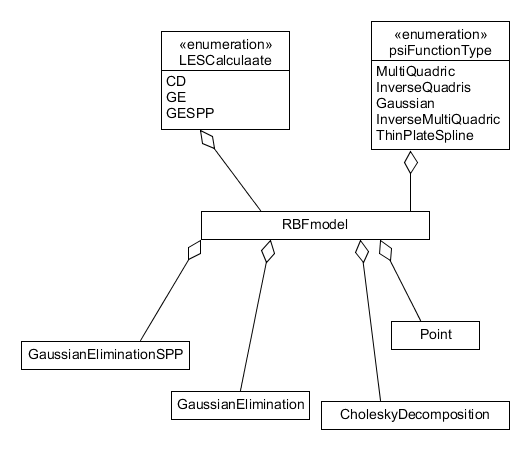
\includegraphics[scale=0.8]{developer/Model.png}
				\caption{Modell réteg osztálydiagramja}
			\end{figure}
		
		
		\subsubsection{Point osztály}
		
			A \textbf{Point} osztály adattagjai közül \textit{x} az $x$, míg  \textit{y} az $y$ tengelyen felvett értéket, \textit{h} pedig az ($x,y$) koordinátában felvett hőmérsékleti értéket jelöli. Az osztály konstruktora \textbf{Point}. A konstruktor három \texttt{int} típusú paramétere adódik át az adattagoknak, ezekben tárolja a pont értékeket.
			
		\subsubsection{CholeskyDecomposition osztály}
		
			Ez az osztály Cholesky-felbontásban számolja az egyenletrendszer megoldását. Az \ref{sssec:num1}. fejezetben leírt módszer algoritmusa került implementálásra, amely a konstruktorban végre is hajtódik. A konstruktor két bemenő paramétert vár. Ezek típusa \texttt{double[,]} kétdimenziós tömb, amely az együttható mátrix, illetve egy \texttt{double[]} tömb, a lineáris egyenletrendszer eredményvektora. Ehhez szükséges egy mátrixtranszponáló függvény, amely az alsó háromszögmátrix transzponálására szolgál, ez a \textbf{Transpose} nevet viseli. Bemenő paramétere egy \texttt{double[,]} típusú két dimenziós tömb, egyben a függvény típusa is. Tartalmaz egy függvényt, mely a példányosítás után meghívható \textbf{GetX} névvel. A függvény \texttt{double[]} típusú tömböt ad vissza értékül, amely az egyenletrendszer megoldása, melyet egy azonos típusú privát adattagban tárolunk, ez a konstruktor meghívásakor számolódik.  
			
		\subsubsection{GaussianElimination osztály}
			
			A Gauss-elimináció algoritmusának megvalósítását ezen osztályon belül végezzük, ahol a konstruktor paraméterei az előzővel azonosak, az osztály szintén tartalmaz egy privát $x$ adattagot, és egy \textbf{GetX} függvényt, melynek visszatérési értéke az előzőével azonos. A konstruktorban számoló algoritmust \cite{gaussian} forrásban lévő algoritmus szerint valósítottam meg. Az osztály abban az esetben, ha $0$ értékkel találkozik a hányados nevezőjében, a \textit{GaussianEliminationSPP} osztályt hívja segítségül, amelynek ez már nem okoz problémát például a \textit{thin plate spline-ok} együtthatómátrixánál.
		
		\subsubsection{GaussianEliminationSPP osztály}
		
			A \textbf{GaussEliminationSPP} osztály az előzővel azonos függvényt és adattagot  tartalmaz, az algoritmus a \cite{gaussian} oldalon lévő \textit{Scaled Partial Pivoting} algoritmus szerint valósítottam meg, amely a részleges főelem kiválasztást jelenti.
			
		\subsubsection{RBFmodel osztály}%
		
			Az \textbf{RBFmodel} osztály konstruktor \texttt{IRBFPersistenceDataAccess} típusú bemenő attribútuma a perzisztencia rétegben lévő interfész amit a kapcsolunk az osztályhoz, a privát \textit{\_dataAccess} szintén azonos típussal rendelkező adattagban tároljuk.
			
			Az osztályhoz tartozó privát adattagok közé tartozik a \texttt{LESSolve}, amely a \texttt{LESCalculate} felsorolóosztály egy tagját tárolja. Ennek kezdőértéke a jelenlegi osztály példányosításakor \textit{GE}, amely a gauss-elimináció rövidítése. Ezt az értéket \textbf{ChangeFT} nyilvános metódus segítségével tudjuk  változtatni, melynek paramétere szintén a felsoroló osztálybeli. Másik a \textit{BasisFunctionType}, ami a bázisfüggvény típusára vonatkozik, melyeket a \texttt{psiFunctionType} felsoroló osztály értékei közül választunk, hozzá tartozó eljárás, mely az értékét változtatja a \textbf{ChangeRBFType}, mely ezen felsoroló osztálybeli paraméterrel rendelkezik. Alapértelmezett értéke \textit{Gaußian}. 
			 
			Az \textbf{AddPoint} az osztályhoz tartozó metódus, amely három paraméterrel rendelkezik. Mindhárom \texttt{double} típusú, a \textbf{Point} osztályhoz szükséges változóértékek. A metódus hozzáadja a pontot a \textit{points} listához, ha az még nem létezett benne, vagy nincs egy másik ponttól való 10 pixelnyi távolságon belül. Amennyiben a \textit{points} lista nincs példányosítva mivel a pontok száma nulla, abban az esetben példányosítja. Ennek a metódusnak a párja a \textbf{RemovePoint} függvény, amelynek visszatérési értéke logikai \texttt{bool} típus, ez a későbbiekben lesz fontos. Amennyimen sikerül eltávolítani híváskor a pontot, \textit{igaz} értékkel tér vissza. Ellenkező esetben pedig \textit{hamissal}.
			
			A \textbf{NewMap} metódus paraméter nélküli eljárás, amely a \textit{localMinimum} és \textit{localMaximum} privát adattagokban lévő értéket visszaállítja a kezdőértékre, a \textit{points} tömböt és ha aktuálisan volt kijelölt pont, mindkettőt felszabadítja.
			
			Pontok módosítására három eljárást alkalmazhatunk. Ezek az eljárások visszatérési érték nélküliek, illetve a \textbf{PointIncrease} és \textbf{PointDecrease} metódusok, melyek közül az első a kiválasztott pont értékét növeli, a második csökkenti, nem rendelkeznek bemenő paraméterrel az adott pont melynek értékét módosítani kell a \textit{\_choosedPoint} adattagban tárolt pont. A harmadik metódus \textbf{PointValue} amely egy egész bemenő értékkel rendelkezik, amely a kívánt hőmérsékleti érték. Ezt adjuk át szintén a \textit{\_choosedPoint-tal} megegyező koordinátákkal rendelkező pontnak, amennyiben van kiválasztott pont.
			
			A függvényértékeket számító metódusokhoz tartozik a \textbf{CalculateMatrix} eljárás, amely nem rendelkezik bemenő paraméterrel. Megalkotja az interpolációs mátrixot, melyben minden pontpárra meghívja a \textbf{Phi} függvényt, amely 3 bemenő paraméterrel rendelkezik. A két első Point, míg a harmadik \texttt{psiFunctionType} típusú attribútum. A függvényben itt vannak implementálva a bázisfüggvények. Ehhez használjuk az osztály \textit{epsilon} adattagját, amely az alakparaméter epszilonnak felel meg, és az \textbf{EuclideanNorm} double visszatérési értékű függvényt, amelynek egy pont a bemenő paramétere és nevének megfelelően az euklideszi normát számítja. A \textbf{CalculateMatrix} eljárás végül meghívja és \textit{w} adattagnak értékül adja a \textbf{LinearEquationSystemCalculate} függvényt, amely a három egyenletrendszert megoldó algoritmus közül meghívja az aktuálisan kiválasztottat. 
			
			A \textbf{FunctionValue} metódus segítségével tudjuk meg egy szükséges pontra az interpolációs függvény értékét, erre az alábbi eljárásokban lesz szükség. A magasabb rétegekben lévő vásznak számításához szükséges függvényekhez szükségünk lesz a függvényértékek maximumára, illetve minimumára. Ehhez használjuk a \textbf{FindlocalMaximumandMinimum} függvényt, melynek visszatérési értéke double[] tömb, melynek első értéke a minimumérték, második a maximumérték. A függvényfolytonosságtól függően, melyet a \textit{cab} adattagban tárolunk, számítjuk a kerekített, vagy pontos függvényértéket az adott pixelen. A \textbf{GetColors} függvény \textit{System.Windows.Media.Imaging} névtérben lévő \texttt{WriteableBitmap} típusú függvény. Két bemenő egész értékű paraméter szélesség és magasság, amely egy fentről érkező vászon méreteinek felelnek meg. A későbbiekben is használatos \textit{pixels1d} egydimenziós \texttt{byte} típusú elemeket tartalmazó tömbbe mentjük el a színeket. Az \textit{fxy} lokális változóba számoljuk hogy az \textit{i}-edik sorban, és egyben ciklusiterációban \textit{i} milyen messze található a vászon tetejétől. Ez alapján színezi a vásznat a függvény. Mivel a \textbf{GetMap} metódus által számolt kép színskálájának ábrázolásához használjuk ezt a függvényt, így a már abban egyszer lefutó \textbf{FindlocalMaximumandMinimum} függvény értékeit használjuk, a korábban már említett \textit{localMaximum}, illetve \textit{localMinumum}-ban eltárolva. Így nem kell kétszer végigmenni a térképen hogy ezt az értéket tudjuk. Jelenlegi kódban ez gondot nem okot, esetleges továbbfejlesztésnél erre viszont figyelni kell. A \textbf{GetMap} függvény szintén \texttt{WriteableBitmap} típusú, és előzővel azonos bemenő paraméterekkel rendelkezik. Amennyiben nincsenek lehelyezett pontjaink \textit{null} értékkel tér vissza. Ellenkező esetben viszont kiszámolja a lineáris egyenletrendszert, a lokális minimum és maximum értéket, Majd az előző függvénnyel közel azonos módon konstruálja meg a bitmapot. Eltérés az \textit{fxy} változó számolásában van. Az adott ponton lévő függvényértéket a folytonos függvény esetén \textbf{FunctionValue}-t jelenlegi ciklusiterációk \textit{i}, illetve \textit{j} értékével hívjuk meg. Nem folytonos esetben kerekítjük az értéket. A \textbf{WritePoints} függvény berajzolja a pontokat a tömbbe. A \textbf{SelectedPoint}, pedig a kiválasztott pontot színezi szürkére, és a \textit{\_choosedPoint} értékét ráállítja a pontra. A \textbf{GetThreeDMap} függvény két feladatot lát el. Első sorban kirajzolja a koordináta rendszert melybe a háromdimenziós ábrázolását tesszük a közelítőfüggvénynek. Tengelyenként ezt külön teszi meg az algoritmus. Ezután kiszámítjuk a függvényt, és elhelyezzük a vászonhoz szükséges tömbben.
			
			A mentésekkel foglalkozó eljárásokat három fele választhatjuk. Az első kettő a színek, illetve mentésével és betöltésével foglalkozik. A \textbf{LoadColors} eljárás, mely egy fájl elérési útvonalát tartalmazza egyetlen paramétereként, ha nincs csatlakoztatott adatkapcsolat, abban az esetben visszatér, és nem kéri be a színeket, ha viszont megfelelően kapcsoltuk a perzisztenciát, akkor a colorize privát színeket tartalmazó listába betölteti a fájlt. A \textbf{LoadPoints} törli a léterő pontokat, majd új listát készít a betöltött pontokból, ezután meghívja a korábban leírt \textbf{CalculateMatrix} eljárást. A \textbf{SaveColors}, illetve \textbf{SavePoints} eljárások a colorize és points listákat adják át a perzisztencia megfelelő metódusainak. Mindkét eljárás bemenőparaméterként a fájl elérési útvonalát névvel együtt kapják meg. A \textbf{saveMap} eljárás másként működik mint az előző két esetben lévő mentés. Két bemenő paramétere közül az első a \texttt{Canvas} típusú vászon, melyet a későbbiekben láthatunk, hogy a kirajzoltatott térkép. Második attribútum az előzőkkel azonos karakterlánc amely szintén az útvonalat tartalmazza. 
			
			
		
		\subsection{Perzisztencia réteg osztályai}
		
			\begin{figure}[ht]
				\centering
				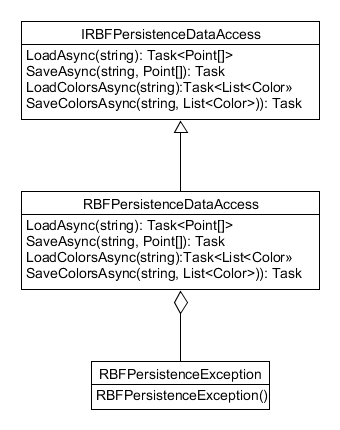
\includegraphics[scale=0.7]{developer/Persistence.png}
				\caption{Perzisztencia réteg osztálydiagramja}
			\end{figure}
		
			\subsubsection{IRBFPersistenceDataAccess interfész}
			
				A réteghez tartozó interfész, amely összeköttetést tud létesíteni más osztályokkal, jelen esetben a modell rétegben lévő \textbf{RBFmodel} osztállyal, az Interfészben deklarált eljárások segítségével. Jelen esetben 4 aszinkron eljárás a LoadAsync, SaveAsync, LoadColorsAsync, és a SaveColorsAsync, melyeket a következő alfejezetben fejtek ki, ahol a definíciójuk is található.
				
			\subsubsection{RBFPersistenceDataAccess osztály}
			
				A \textbf{LoadAsync} eljárásban \textit{StreamReader} osztály segítségével olvassuk be aszinkron a sorokat. Ez azt jelenti hogy minden sor külön szálként olvasódik be, ezzel gyorsítjuk a beolvasást. Ezután eltároljuk a számokat, amiket a sorok felszeletelésével kapunk. Beletesszük a kapott számokból megkonstruált pontot a tömbbe, amelyet a végén visszaadunk. 
				
				A \textbf{SaveAsync} eljárás a pontok mentését végzi. \textit{StreamWriter} osztály segítségével nyitjuk meg az írandó fájlt. A megnyitás után a pontok adattagjait szóközökkel elválasztva írjuk fájlba.
				
				A \textbf{LoadColorsAsync} eljárásban a színskálát töltjük be fájlból. Amint a fájlban szereplő számok száma nem éri el a 8-at, akkor hibát dobunk, mivel a színskálát nem tudjuk felállítani két szín nélkül. Szintén a \textit{StreamReader} beépített osztály segítségével végezzük a beolvasást.
				
				A \textbf{SaveColorsAsync} eljárásban a színskálának a mentését végezzük. A kimenő listának színeinek adattagjait egyesével vesszük, karakterlánccá konvertáljuk. Az adattagokat \textit{BGRA} sorrendben írjuk ki a fájlba szóközzel elszeparálva.
				
				A most leírt eljárások mindegyikében szerepel a ,,try-catch'' szerkezet, kivételkezelés céljából. Amint nem sikerül a betöltés valami miatt, vagy az említett hosszprobléma miatt a  z eljárás kivétellel tér vissza, amit a modell rétegben le tudunk kezelni.
				
			\subsubsection{RBFPersistenceException osztály}
			
				\textbf{Exception} osztályból leszármaztatott osztály, melyet a hiba elkapásánál használunk, és az előző alfejezetben definiált eljárások alatt keletkező hiba esetén dobjuk.
				 
		\subsection{Nézet-modell réteg osztályai}
			
			\begin{figure}[ht]
				\centering
				\includegraphics[scale=0.7]{developer/ViewModel.png}
				\caption{Nézet-Modell osztálydiagramja}
			\end{figure}
		
			\subsubsection{MessageEventArgs osztály}
			
				Az \textbf{EventHandler} metódushoz szükséges, az üzenetet tartalmazza. Privát adattagja karakterlánc típusú. 
				
			\subsubsection{ViewModelBase osztály}
			
				Az osztály számunkra nagyon fontos. Ebben található az \textbf{OnPropertyChanged} metódus, amely jelzi hogy valamelyik számunkra szükséges adattag változott. Illetve itt található az \textbf{EventHandler} metódus is ami az eseménykezelés fontos eljárása. Mindhárom saját nézet-modell osztályt ebből származtatjuk le.
				
			\subsubsection{DelegateCommand osztály}
			
				A nézetet köti a nézet-modell rétegben lévő osztályainkhoz. Ezeken keresztül küldjük át az egyes gombok, vagy menüpontok által kiváltott eseményeket. 
				
			\subsubsection{ThreeDVM osztály}
			
				A \textbf{ThreeDVM} osztály példányosításkor paraméterként kapja a hozzá tartozó nézet rétegbeli \textbf{ThreeDView} ablakot. Ezt eltároljuk a \textit{\_view} privát adattagban, illetve megkapja a modellünket, ami segítségével számítja a felületre rajzolandó vásznat. Egyetlen eljárása az osztálynak a \textbf{DrawFunction} nevet viseli. Ennek futása alatt a kurzort töltő ikonra állítjuk. Lekérdezzük a képet, majd a \textit{\_view}-hoz tartozó canvashoz adjuk. Ezután felcímkézzük a koordinátatengelyeket, Majd a $Z$ tengelyen lévő skálát is felcímkézzük. A tengelycímkéknél félkövér stílust használunk a jobb láthatóság érdekében.
				
			\subsubsection{ColorScaleViewModel osztály}
			
				A \textbf{ColorScaleViewModel} osztályt összekapcsoljuk a \textbf{ColorScaleWindow}-val ezt a nézet \textit{DataContext} adattagjával tesszük, hozzákötjük a nézet-modellünket. Példányosításkor a modellünket kapjuk, amelyet ezután a \textit{\_model} privát adattagban tárolunk el. Szükségünk lesz továbbá színek listájára \textit{Colors} néven, amit majd a táblázathoz használunk. \textit{SelectedColor} egy publikus adattag, ami a táblázatban kiválasztott elemnek felel meg. Változáskor \textit{OnPropertyChanged} eljárást hívjuk meg. \textbf{LoadData} eljárás végig iterál a modellünk \textbf{colorize} adattagján, amely a színeket tárolja. Ezeket belepakolja a \textbf{Colors} jelenlegi listába, ami után szintén kiváltjuk az \textit{OnPropertyChanged} metódust. Amennyiben nem sikerült az eljárást végrehajtani, az \textbf{OnMessageApplication} ViewModelBase osztálybeli metódussal üzenjük meg a felhasználónak, hogy ,,Váratlan hiba történt!''. 
				
				A módosító metódusok találhatók az osztály alján, amelyeket az ablakon lévő gombok megnyomásakor kiváltódó \textit{DelagateCommand}-ok segítségével érünk el. \textbf{Modify} eljárás a színmódosításkor hívandó metódus. Színek választásánál nagy segítség a \textbf{ColorDialog} osztály aminek egy példányát használjuk, a színválasztáshoz. Amennyiben a szín már korábban létezett a skálában, nem módosítjuk azt, ellenkező esetben pedig a kiválasztott elemet változtatjuk meg. Az \textbf{Add} eljárás az előzővel azonos színválasztó ablakban kiválasztott szín ellenőrzése után, ha az nem szerepel a listában, beszúrja a végére. A \textbf{Delete} metódus lefutáskor ellenőrzi hogy a jelenlegi listában több elem van-e mint $2$. Amennyiben nem a metódus nem fut végig. Ha több elem található abban az esetben a kijelölt elemet eltávolítja a listából.
			
			\subsubsection{RBFViewModel}
			
				Az \textbf{RBFviewModel} osztályt \textbf{MainWindow} ablakkal kapcsoljuk össze. A \textbf{ViewModelBase} osztályból származtatunk. A konstruktor 2 bemenő paraméterrel rendelkezik. Ebben inicializáljuk a két paramétert, eltároljuk a \textit{\_view} és \textit{\_model} privát adattagokban. A \textbf{DelegateCommand} típusú vezérlőinket, melyeket a konstruktor előtt deklaráltunk, szintén itt csatoljuk az adattagokhoz. Ezeket négy részre lehet bontani. Az elsőbe tartozik a számítási típusokat kiválasztó parancsok. Ezek körébe sorolható a függvényfolytonosság, az epszilon értékének megválasztása, a bázisfüggvény típusa, és a lineáris egyenletrendszer megoldó módszer választása. 
				
				A menüpontok előtti kijelölés egyszerű eltávolításához használjuk a \textbf{BfTypeUnchecked}, \textbf{FTypeUnchecked}, \textbf{ETypeUnchecked}, \textbf{EUnchecked} metódusokat. 
				
				A \textbf{SelectedPoint} kiválasztott pontot színezteti a modellel szürkére. Amennyiben van pont kiválasztva, a nézet jobboldalára írja ki annak adatait. Ellenkező esetben nem ír ki adatot. A \textbf{RefreshMap} eljárás paraméter nélküli, és a nézet fővásznát, illetve a hozzá tartozó skálát frissíti, azokat címkéire írja a skálát. Az \textbf{askBox} metódusban kérdezzük meg a felhasználót arról hogy mit kíván tenni új térkép kezdése előtt. A három lehetséges esetet szétválasztjuk. Az ,,Igen'' esetén mentjük a pontokat, ,,nem'' választásánál viszont csak egyszerűen új vásznat készít a metódus.  
				 
				Az eliminációs módszerek cseréjéhez a \textbf{ChangeFT}, a bázisfüggvény választásnál a \textbf{ChangeType}, függvényfolytonosságnál a \textbf{CAB} segéd  metódust használjuk.
				
				A pontok beszúrásánál \textbf{PointPaste} metódus hívódik meg. Ekkor a vásznon vett pozíciónk helyére leszúrja a pontot a program. A Pontnak törlését a \textbf{PointRemove} metódus végzi. Amint sikerült eltávolítania a pontot, abban az esetben frissíti a térképet. A színskála megválasztásánál a \textbf{SetColors} metódusba nyitjuk megy a \textbf{ColorScaleWindow}-ot és adjuk a \texttt{DataContext}-jének a \textbf{ColorScaleViewModel} osztályt.
				
				A mentések körébe tartozik a \textbf{SaveImage} eljárás, amely megkérdezi hova mentse a \texttt{.png} kiterjesztésű fájlt. A pontok mentésére szolgál a \textbf{SaveData} eljárás, azoknak betöltésére pedig a \textbf{LoadData} metódus. A színskálák mentésére a \textbf{SaveColorData}, illetve a \textbf{LoadColorData} metódusok szolgálnak.
				
		\section{Tesztelés}
		
			Az alábbi alfejezetben a program helyes futásáról győződhetünk meg. Különválasztjuk a fehér-doboz és fekete-doboz tesztelést. Mindkét tesztelési formának megvan az előnye. A fehér-doboz teszteléssel a modellünk algoritmusainak működését vizsgáljuk, míg a feketével azt nézzük hogy a tervezésben leírtak alapján cselekszik-e a programunk a használat során.
			
			\subsection{Fehér-doboz tesztelés}
				Ebben a fejezetben azt fogjuk vizsgálni, hogy a modell megfelelően szolgálja ki a magasabb rétegeinket. A pontokkal foglalkozó metódusokat egységtesztben vizsgáljuk, az eliminációs algoritmusokat pedig összehasonlítás alapján láthatjuk. 
				
				\subsubsection{Egységteszt}
				
					Az egységteszt a program mellett található külön projektben. A projekt egyetlen osztályának konstruktorában példányosítjuk a modellünket, és a tesztosztály eljárásaiban  A pontok kezelésével foglalkozó tesztek megadott véletlenszerű értékekre ellenőriz. A program tesztelése során kritikus értékekkel nem kell számolnunk, a modellnek teljesítenie kell a számítást sokkal nagyobb vásznakra, mint ami egy nagy felbontású monitor felülete. 
					
					\textbf{Ponthozzáadás teszt:} A modellünk \textbf{AddPoint} metódusának tesztjét az azonos elnevezésű eljárásban vizsgáljuk.
					\begin{itemize}
						\item \textsc{1. eset :} Hozzáadunk pontot a metódushoz, ekkor ellenőrizzük hogy a lista hosszát.
						\item \textsc{2. eset :} A pontunk közelébe lehelyeznénk még egy pontot. Ekkor nem bővülhet a lista mert túl közel van a két pont egymáshoz. 
						\item \textsc{3. eset :} Egy megfelelő távolságban lévő pont lehelyezésénél a lista bővül eggyel. 
					\end{itemize}  
				
					\textbf{Ponttörlés teszt:} A modell \textbf{RemovePoint} működését nevével megegyező metódusban tesztelünk le.
					\begin{itemize}
						\item \textsc{1. eset :} Nincs kijelölve pont, ekkor próbálunk törölni. Ebben az esetben nem történik semmi.
						\item \textsc{2. eset :} Kijelölünk egy pontot majd azt töröljük. Ekkor a pontok listája csökken eggyel.
						\item \textsc{3. eset :} A pontkijelölésnek nem szabad eltávolított pontot jelölnie.  
					\end{itemize} 
				
					\textbf{Értéklekérdezés teszt:} A \textbf{Value} értéklekérdező metódust számítását a \textbf{PointValue} osztályban teszteljük.
					\begin{itemize}
						\item Hozzáadunk pontokat a modellhez, majd azokon vett közelítőfüggvény értékét vizsgáljuk, hogy megegyezik-e a pontoknak megadott értékekkel. 
					\end{itemize} 
				
					\textbf{Értéknövelés teszt:} A \textbf{PointIncrease} helyességét, a \textbf{PointIncreasing} eljárásban vizsgáljuk.
					\begin{itemize}
						\item Hozzáadott pontoknál egyik pont értékét növeljük, majd megnézzük, hogy értéke eggyel nagyobb, mint a növelés előtti. 
					\end{itemize} 
				
					\textbf{Értékcsökkentés teszt:} A \textbf{PointDecrease} helyességét, a \textbf{PointDecreasing} eljárásban vizsgáljuk.
					\begin{itemize}
					    \item Hozzáadott pontoknál egyik pont értékét csökkentjük, majd megnézzük, hogy értéke eggyel kisebb, mint a növelés előtti. 
					\end{itemize} 
				
					\textbf{Értékmegadás teszt:} A pont értékének változtatását a \textbf{PointValue} függvénnyel érhetjük el. Ennek tesztelését a \textbf{PointValueChoose} eljárásban végezzük.
					 \begin{itemize}
					 	\item Hozzáadott pontoknál egyik pont értékét megváltoztatjuk, majd megnézzük, hogy értéke megegyezik-e a kívánt értékkel.
					 \end{itemize} 
			 	
			 	
			 	\subsubsection{Összehasonlító tesztelés}
			 		Az összehasonlítást online számítások és a saját programom számítása közt végezzük. Mindhárom saját felbontásra ugyanaz az eredmény jött ki, így nem különböztetem meg a módszereket tesztelésnél. Az online programban \cite{wolframalpha} ismertsége miatt meg lehet bízni.
			 		
			 		A pontokat véletlenszerűen vettem fel a vásznon, azokhoz tartozó fí értékek kerülnek a megoldandó egyenletrendszer mátrixába. A programot Debug módban fogom meg a lépéseknél ekkor a bemenő adatokat látjuk.
			 		\begin{figure}[ht]
			 		 	\centering
			 		 	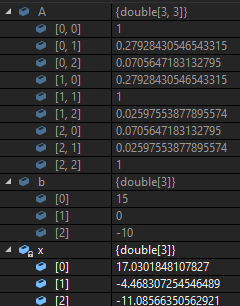
\includegraphics[scale=1]{developer/test1.png}
			 		 	\caption{Tesztértékek a lineáris egyenletrendszer megoldásánál}
		 		 	\end{figure}
	 		 	
	 		 		Az adatokat manuálisan beírva a webes alkalmazásba a következő eredményt kapjuk.
	 		 		\begin{figure}[ht]
	 		 			\centering
	 		 			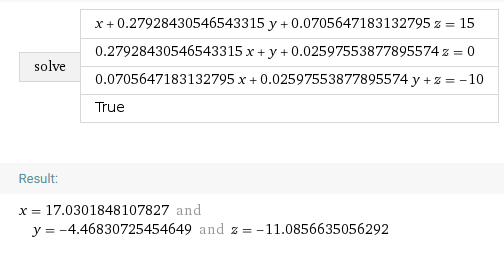
\includegraphics[scale=1]{developer/test1real.png}
	 		 			\caption{Tesztértékek számítása webes felületen}
	 		 		\end{figure}
 		 		
 		 			Az összehasonlításban látható hogy nincs eltérés, sőt a miénk egy tizedesjeggyel pontosabb számot adott. 
			 \subsection{Fekete-doboz tesztelés}
			 	Fekete-doboz teszteléssel nem konkrét algoritmusokat tesztelünk, hanem hogy a program helyes működést biztosít-e a felhasználónak. Ehhez ismételten már létező hőtérképeket veszünk alapul. Az időkép \cite{idokep} oldalán található mai nap hőmérsékleti térképét hasonlítjuk össze a programunk által generált hőtérképpel.
			 	
			 	\begin{figure}[ht]
			 		\centering
			 		\includegraphics[scale=0.5]{developer/today.png}
			 		\caption{Magyarország hőtérképe 2019.12.04-én}
			 	\end{figure}
		 		\begin{figure}[hb]
		 			\centering
		 			\includegraphics[scale=0.4]{developer/todaymyprogram.png}
		 			\caption{Magyarország hőtérképe saját közelítésünk szerint}
		 		\end{figure}
	 			
	 			Látható a két ábrán hogy kis eltérés van a színskálázásnál, de a színátmenetek hasonlóak a két kép között. A lehelyezett pontok mennyisége elegendő a jó közelítéshez, viszont mivel sokkal kevesebb felvett pontunk van, így az átmenetek nem olyan élesek mint az Időkép hőtérképén.
	 			
	 			Továbbfejlesztési lehetőségek megvalósítását bármely olvasónak ajánlom, és esetleges megkeresését várom, amennyiben bármi kérdése felmerül a programmal kapcsolatban.